%\pdfoutput=1 % only if pdf/png/jpg images are used
\documentclass{article}
\usepackage{amssymb}
%\usepackage[dvips]{graphicx}
\usepackage{graphicx}
\usepackage{verbatim}
\usepackage{xspace}
\newcommand{\E}{EIGER\xspace}  
\begin{document}

\title{\E - short manual}
\date{\today}
\maketitle
\tableofcontents

\section{Usage}

\subsection{Mandatory setup - Hardware}
An EIGER single module (500~kpixels) needs:
\begin{itemize}
\item A chilled (water+alcohol) at approximately 21~$^{\circ}$C, which needs to dissipate 85~W.
\item A power supply (12~V, 8~A).
\item 2$\times$1~Gb/s Ethernet connectors to control the detector and, optionally, receive data at low rate. A DHCP server that gives IPs to the 1~Gb/s connectors of the detector is needed. Note that flow control has to be enabled on the switch you are using.
\item 2$\times$10~Gb/s transceivers to optionally, receive data at high rate.
\end{itemize}
The equipment scales linearly with the number of modules.
Figure~\ref{fig:1} shows the relationship between the \textbf{Client} (which sits on a beamline control PC), the \textbf{Receiver} (which can run in multiple instances on one or more PCs which receive data from the detector. The receiver(s) does not necessary have to be running on the same PC as the client.) It is important that the receiver is closely connected to the detector (they have to be on the same network). Note that if you implement the 1Gb/s redout only: client, receiver and detector have to be all three in the same network. If you omplement teh 10Gb/s redout, then client, the 1~GbE of the detector and the receiver have to stay on the 1GbE. But the receiver data receiving device and the 10GbE detector can be on their private newtwork, minimising the missing packets.  

\begin{figure}[t]
\begin{center}
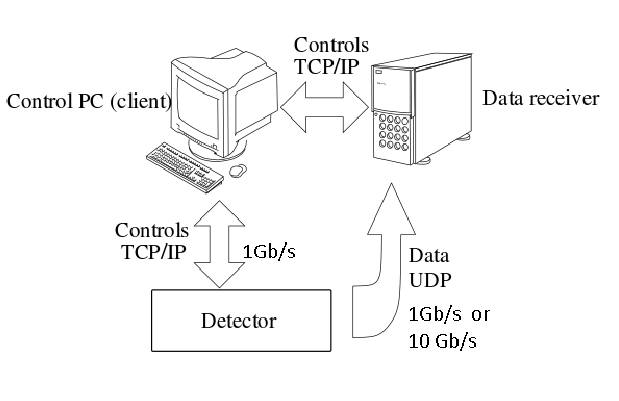
\includegraphics[width=.8\textwidth]{Client2}
\end{center}
\caption{Communications protocol between the Client PC, the receiver pc and the detector.}
\label{fig:1}
\end{figure}

The Client talks to control over 1~Gb Ethernet connection using TCP/IP to the detector and to the receiver. The detector sends data in UDP packets to the receiver. This data sending can be done over 1~Gb/s or 10~Gb/s. 
 

\subsection{Mandatory setup - Receiver}

The receiver is a process run on a PC closely connected to the detector. Open one receiver for every half module board (remember, a module has two receivers!!!) . Go to {\tt{slsDetectorsPackage/bin/}}, \textbf{slsReceiver} should be started on the machine expected to receive the data from the detector.

\begin{itemize}
\item {\tt{./slsReceiver --rx\_tcpport xxxx}} 
\item {\tt{./slsReceiver --rx\_tcpport yyyy}}
\end{itemize}
where xxxx, yyyy are the tcp port numbers. Use 1955 and 1956 for example. Note that in older version of the software {\tt{--mode 1}} was used only for the ``bottom'' half module. Now, the receiver for the bottom is open without arguments anymore, but still in the configuration file one needs to write {\tt{n:flippeddatax 1}}, where {\tt{n}} indicated the half module number, 1 if it is a module.
\\ Open as many receiver as half module boards. A single module has two half module boards.

\subsection{Mandatory setup - Client}

\underline{In the case of cSAXS, the detector software is installed on the x12sa-ed-1 machine:}\\
\underline{/sls/X12SA/data/x12saop/EigerPackage/slsDetectorsPackage}

The command line interface consists in these main functions:
\begin{description}
\item[sls\_detector\_acquire] to acquire data from the detector
\item[sls\_detector\_put] to set detector parameters
\item[sls\_detector\_get] to retrieve detector parameters
\end{description}

First, your detector should always be configured for each PC that you might want to use for controlling the detector. All the examples given here show the command {\tt{0-}}, which could be omitted for the EIGER system $0$. In the case more EIGER systems are controlled at once, the call of {\tt{1-}},.. becomes compulsory.

To make sure the shared memory is cleaned, before starting, one should do:  
\begin{verbatim}
sls_detector_get 0-free
\end{verbatim}
To do that:
\begin{verbatim}
sls_detector_put 0-config mydetector.config
\end{verbatim}
Refer to sample configuration files to produce the appropriate one for your detector.
\underline{In the case of cSAXS the {\tt{mydetector.config}} *at present* is:}\\ 
\underline{/sls/X12SA/data/x12saop/EigerPackage/beb\_1.5M\_1Gb\_fiber.config}

One can configure all the detector settings in a parameter file {\tt{setup.det}}, which is loaded by doing:
\begin{verbatim}
sls_detector_put 0-parameters setup.det
\end{verbatim}

In the case of \E, the proper bias voltage of the sensor has to be setup, i.e. the {\tt{setup.det}} file needs to contain the line {\tt{vhighvoltage 150}}. Other detector functionality, which are rarely changed can be setup here. 
Other important settings that are configured in the {\tt{setup.det}} file are:
\begin{itemize}
\item {\tt{tengiga 0/1}}, which sets whether the detector is enabled to send data through the 1~or the 10~Gb Ethernet.
\item {\tt{flags parallel/nonparallel}}, which sets whether the detector is set in parallel acquisition and readout or in sequential mode. This changes the readout time of the chip and affects the frame rate capability (faster is {\tt{parallel}}, with higher noise but needed when the frame rate is $>2$~kHz. 
\item {\tt{dr 32/16}} sets the detector in autosumming mode (32 bit counter or not autosumming, 12 bit out of the chip). This is strictly connected to what is required for the readout clock of chip. See next point.
\item {\tt{clkdivider 0/1/2}}. Changes the readout clock: 200, 100, 50~MHz. Note that autosumming mode ({\tt{dr 32}} only works at {clkdivider 2}). By selecting Refer to readout timing specifications in~section\ref{timing} for how to set the detector. 
\item {\tt{flags continuous/storeinram}}. Allows to take frame continuously or storing them on memory. Normally {\tt{continuous}} should be used. Enabling the  {\tt{stroreinram}} mode allows you to obtain the maximum frame rate, but at the expenses to have to receive the data all at the end of the acquisition. Refer to readout timing specifications in section~\ref{timing} for how to set the detector.
\end{itemize}

One should notice that, by default, by choosing the option {\tt{dr 32}}, then the software automatically sets the detector to  {\tt{clkdivider 2}}. By choosing the option {\tt{dr 16}}, the software automatically sets the detector to  {\tt{clkdivider 1}}. One needs to choose {\tt{clkdivider 0}} after setting the {\tt{dr 16}} option to have the fastest frame rate. 
We would recommend expert users (beamline people) to write their parameters file for the users. 

\section{Setting up the threshold}
\begin{verbatim}
sls_detector_put 0-trimen N xxxx yyyy zzzz
sls_detector_put 0-settings [veryhighgain/highgain/standard/lowgain/verylowgain]
sls_detector_put 0-threshold energy_in_eV
\end{verbatim}
The first line requires to specify how many ({\tt{N}}) and at which energies in eV {\{tt{xxxx}}, {\tt{yyyy}}, {\tt{zzzz}} and so on) the trimmed files were generated (to allow for an interpolation). This line should normally be included into the {\tt{mydetector.config}} file and should be set for you by one of the detector group.
NORMALLY, in this new calibration scheme, only {\tt{settings standard}} will be provided to you. Unless specific cases to be discussed.
The threshold at 6000 eV , for example would be set as:{\tt{sls\_detector\_put 0-threshold 6000}}.

\section{Standard acquisition}

After you setup the setting and the threshold, you need to specify the exposure time, the number of real time frames and eventually how many real time frames should be acquired:
\begin{verbatim}
sls_detector_put 0-exptime 1[time_is_s]
sls_detector_put 0-frames 10
sls_detector_put 0-period 0[time_is_s]
\end{verbatim}
In this acquisition 10 consecutive 1~s frames will be acquired. Note that {\tt{period}} defines the sum of the acquisition time and the desired dead time before the next frame. If {\tt{period}} is set to 0, then the next frame will start as soon as the detector is ready to take another acquisition. \\

For \E, at the moment 5 settings are possible: {\tt{standard}}, {\tt{lowgain}}, {\tt{verylowgain}}, {\tt{veryhighgain}} and {\tt{highgain}}. According to the setting chosen, one can reach different energies. Refer to the settings requirements for your detector.\\ 
Notice that the option {\tt{settings standard/highgain/lowgain/veryhighgain/verylowgain}} actually loads the trimbit files so it is time consuming. Only setting the {\tt{threshold}} does not load trimbit files.  

The threshold is expressed in (eV) as the proper threshold setting, i.e. normally is set to 50\% of the beam energy.  

\underline{At cSAXS, the {\tt{settingsdir}} and {\tt{caldir}} are in}\\\underline{/sls/X12SA/data/x12saop/EigerPackage/calibrations/}\\ 

You need to setup where the files will be written to
\begin{verbatim}
sls_detector_put 0-outdir /scratch
sls_detector_put 0-fname run
sls_detector_put 0-index 0
\end{verbatim}
this way your files will all be named /scratch/run\_dj\_i.raw where $j$ is relative to each specific half module, $i$ in the {\tt{index}} starts from 0 when starting the detector the first time and is automatically incremented. The next acquisition {\tt{index}} will be 1. One can reset the  {\tt{index}} to what wished.

To acquire simply type:
\begin{verbatim}
sls_detector_acquire 0-
\end{verbatim}
Note taht acquiring is blocking.

There is a more complex way of performing an acquisition, that is useful for debugging and in case one wants a non blocking behaviour: 
\begin{itemize}
\item {\tt{sls\_detector\_put 0-receiver start}} 
\item {\tt{sls\_detector\_put 0-status start}} 
\end{itemize}

You can poll the detector status using:
\begin{verbatim}
sls_detector_get 0-status 
\end{verbatim}
If the receiver has not yet received the finished signal by the detector, the answer will return {\tt{running}}. If the detector has finished and ready for the next acquisition, then it will return {\tt{idle}}.
The detector will not accept other commands while acquiring. If an acquisition wishes to be properly aborted, then:
\begin{itemize}
\item {\tt{sls\_detector\_put 0-status stop}} 
\end{itemize}
this same command can be used after a non proper abortion of the acquisition to reset to normal status the detector.

\section{Readout timing- maximum frame rate}\label{timing}
IMPORTANT: to have faster readout and smaller dead time, one can configure {\tt{clkdivider}}, i.e. the speed at which the data are read, i.e. 200/100/50~MHz for {\tt{clkdivider 0/1/2}} and the dead time between frames through {\tt{flags parallel}}, i.e. acquire and read at the same time or acquire and then read out.
The configuration of this timing variables allows to achieve different frame rates. NOTE THAT IN EIGER, WHATEVER YOU DO, THE FRAME RATE LIMITATIONS COME FROM THE NETWORK BOTTLENECK AS THE HARDWARE GOES FASTER THAN THE DATA OUT.

In the case of REAL CONTINUOUS readout, i.e. continuous acquire and readout from the boards (independent on how the chip is set):
\begin{itemize}
\item 1~GbE, {\tt{dr 16}}, {\tt{flags continous}}, \textbf{256~Hz} 
\item 1~GbE, {\tt{dr 32}}, {\tt{flags continous}}, {\tt{clkdivider 2}}, \textbf{128~Hz}
\item 10~GbE, {\tt{dr 16}}, {\tt{flags continous}}, {\tt{flags parallel}},{\tt{clkdivider 0}}, \textbf{2.56~kHz}  
\item 10~GbE, {\tt{dr 32}}, {\tt{flags continuous}}, {\tt{clkdivider 2}}, \textbf{1.28~kHz}  
\item 10~GbE, {\tt{dr 8}}, {\tt{flags continous}}, {\tt{flags parallel}},{\tt{clkdivider 0}}, \textbf{5.12~kHz}
\item 10~GbE, {\tt{dr 4}}, {\tt{flags continous}}, {\tt{flags parallel}},{\tt{clkdivider 0}}, \textbf{10.24~kHz}
\end{itemize}
Note that in the {\tt{continuous}} mode, some buffering is still done on the memories, so a higher frame rate than the proper real continuos one can be achieved. Still, this extra buffering is possible till the memories are not saturated. 
The number of images that can be stored on memories are:
\begin{table}
\begin{tabular}{|c|c|}
\hline
dynamic range & images\\
\hline
4 & 30000\\
\hline
8 & 15000\\
\hline
16 & 7600\\
\hline
\end{tabular}
\caption{Amount of images that can be stored on board.}
\end{table}

The maximum frame rate achievable with 10~GbE, {\tt{dr 16}}, {\tt{flags continuous}}, {\tt{flags parallel}},{\tt{clkdivider 0}}, \textbf{6.1~kHz}. This is currently limited by the connection between the Front End Board and the Backend board. We expect the 32 bit mode limit to be \textbf{2~kHz} ({\tt{clkdivider 2}}).
 In dynamic range {\tt{dr 8}} the frame rate is \textbf{11~kHz} and for{\tt{dr 4}} is \textbf{22~kHz}. For 4 and 8 bit mode the frame rate are directly limited by the speed of the detector chip and not by the readout boards.    

Here is a list of all the readout times in the different configurations:
\begin{table}
\begin{tabular}{|c|c|c|c|c|}
\hline
dynamic range & clkdivider & mode & readout time ($\mu$s) & max frame rate (kHz)\\
\hline
16 & 0 & parallel & 2.75 & 6\\
\hline
16 & 0 & nonparallel &  126 & 3.4\\
\hline
16 & 1 & parallel &  5.36 & 2.9\\
\hline
16 & 1 & nonparallel & 252 & 1.7\\
\hline
16 & 2 & parallel &  10.6 & 1.5\\
\hline
16 & 2 & nonparallel & 504 & 0.85\\
\hline
32 & 2 & parallel &  10.6 & 2\\
\hline
32 & 2 & nonparallel & 504 & $<2$\\
\hline
\end{tabular}
\caption{Readout settings.}
\end{table}
\textbf{As if you run too fast, the detector could become noisier, it is important to match the detector settings to your frame rate. This can be done having more parameters files and load the one suitable with your experiment.} We experienced that {\tt{highgain}} settings could not be used at 6~kHz.


\section{External triggering options}
The detector can be setup such to receive external triggers. Connect a LEMO signal to the TRIGGER IN connector in the Power Distribution Board. The logic 0 for the board is passed by low level 0$-$0.7~V, the logic 1 is passed to the board with a signal between 1.2$-$5~V. Eiger is 50~$\Omega$ terminated. By default the positive polarity is used (negative should not be passed to the board).  
\begin{verbatim}
sls_detector_put 0-timing [auto/trigger/burst_trigger/gating]
sls_detector_put 0-frames x
sls_detector_put 0-cycles y
sls_detector_acquire 0-
\end{verbatim}
No timeout is expected between the start of the acquisition and the arrival of the first trigger. 

Here are the implemented options so far:
\begin{itemize}
\item {\tt{auto}} is the software controlled acquisition, where {\tt{exptime}} and {\tt{period}} have to be set.
\item {\tt{trigger}} 1 frame taken for 1 trigger. You {\tt{frames}} needs to be  1 always, {\tt{cycles}} can be changed and defines how many triggers are considered. In the GUI this is called trigger exposure series. 
\item {\tt{burst\_trigger}} gets only 1 trigger, but allows to take many frames. With {\tt{frames}} one can change the number of frames. {\tt{cycles}} needs to be 1. In the gui it is called trigger readout.
\item{\tt{gating}} allows to get a frame only when the trigger pulse is gating. Note that in this case the exp time and period only depend on the gating signal. {\tt{cycles}} allows to select how many gates to consider. 
\end{itemize}

Hardware-wise, the ENABLE OUT signal outputs when the chips are really acquiring. This means that the single subframes will be outputted in 32 bit mode. The TRIGGER OUT outputs the sum-up-signal at the moment (which is useless). This will be changed in the future to output the envelop of the enable signal. 

We are planning to change some functionality, i.e. unify the {\tt{trigger}} and {\tt{burst}} trigger modes and make both {\tt{frames}} and {\tt{cycles}} configurable at the same time.

\section{Offline processing and monitoring}
\subsection{Offline image reconstruction}
The offline image reconstruction is in {\tt{slsDetectorsPackage/slsImageReconstruction}}.

The detector writes a raw file per receiver. An offline image reconstruction executable has been written to collate the possible files together and produce cbf files. The executable uses the CBFlib-0.9.5 library (downloaded from the web as it download some architecture dependent packages at installation).\\
\underline{At cSAXS, the CBFlib-0.9.5 has been compiled -such that the required packages are}\\\underline{ downloaded in /sls/X12SA/data/x12saop/EigerPackage/CBFlib-0.9.5.}\\ 

To use it for a single module:
\begin{verbatim}
cbfMaker [filename with dir]
\end{verbatim}
eg.
{\tt{cbfMaker /scratch/run\_63\_d1\_f000000000000\_3.raw}}\\

To use it for a 1.5 multi modules:
\begin{verbatim}
cbfMaker [filename] [pixels x] [pixels y] ([singlemodulelongside_x] [start det])
\end{verbatim}
eg.
{\tt cbfMaker /scratch/run\_63\_d0\_f000000000000\_3.raw  3072 512 1 0}.\\
The {\tt{[singlemodulelongside\_x]}} and {\tt{[start det]}} param are optional. Defaults are ``1'', the detector long side is on the x coordinate and start to reconstruct from module 0. 
The executables: 
\begin{verbatim}
bcfMaker1.5M [file_name_with_dir]
bcfMaker9M [file_name_with_dir]
\end{verbatim}
contain the hardcoded geometry for the 1.5M (3 modules horizontal on the long side) and for the 9M at cSAXS: 6(short side)$\times$3 (long side) modules.\\ 
Missing packets in a frame and border pixels ($\times 2$ and $\times 4$ are given with value $-1$ at the present time.

It is important to know, that the pixels at the edge between 2 chips count more as double size. We can virtually introduced 1 virtual pixel per double larger pixel, so to have an even number of counts everywhere. Virtual pixels (not filled ) between module gaps are also inserted.

 \begin{verbatim}
   GapPixelsBetweenChips_x = 2;
   GapPixelsBetweenChips_y = 2;
   GapPixelsBetweenModules_x = 8;
   GapPixelsBetweenModules_y = 36;
 \end{verbatim}

\subsection{Read temperatures from boards}

With an updated kernel on the linux boards (ask to the SLS detector group for specifications), it is possible to monitor the temperature on the Back End Boards: 
\begin{verbatim}
temp_fpga   #gets the temperature of the fpga
temp_fpgaext   #gets the temperature close to the fpga
temp_10ge   #gets the temperature close to the 10GE
temp_dcdc   #gets the temperature close to the dc dc converter
temp_sodl   #gets the temperature close to the left so-dimm memory
temp_sodr   #gets the temperature close to the right so-dimm memory
temp_fpgafl   #gets the temperature of the left front end board fpga
temp_fpgafr   #gets the temperature of the left front end board fpga

\end{verbatim}

You need to use the command specifying from which board you desire the temperature readings, for example:
\begin{verbatim}
./sls_detector_get 0:temp_fpga
./sls_detector_get 1:temp_fpga
\end{verbatim}

\section{Autosumming and rate corrections}

In the case of autosumming mode, i.e, {\tt{dr 32}}, the acquisition time ({\tt{exptime}} is broken in as many subframes as they fit into the acquisition time minus all the subframes readout times. By default the {\tt{subexptime}} is set to 2.621440~ms. This implies that 12 bit counter of \E will saturate when the rate is above or equal to 1.57~MHz/pixel. The minimum value is of order of 10~ns (although as explained values smaller than 500~$\mu$s do not make sense). The maximum value is 5.2~s.

The subframe length can be changed by the user by doing: 
\begin{verbatim}
sls_detector_put 0-subexptime [time_in_s] 
\end{verbatim}

One needs to realize that the readout time, for each subframe is 10.5~$\mu$s if the detector is in parallel mode. 500~$\mu$s if the detector is in non parallel mode. Note that in {\tt{dr 32}}, as the single frame readout from the chip is 500~$\mu$s, no {\tt{subexptime}}$<$500~$\mu$s can be set in {\tt{parallel}} mode. To have smaller {\tt{subexptime}}, you need the {\tt{nonparallel}} mode, although this will have a larger deadtime than the acquisition time.\\

Online rate corrections can be activated. They are particularly useful and implemented \textbf{only} in the autosumming mode, i.e. when {\tt{dr 32}} is activated as  every single subframe is corrected before summing it. To correct for rate, the subframe duration has to be known to the correction algorithm.    
To activate the rate corrections, one should do:\\
\begin{verbatim}
sls_detector_put 0-ratecorr [tauval_in_ns]
\end{verbatim}
To deactivate:
\begin{verbatim}
sls_detector_put 0-ratecorr 0
\end{verbatim}
Default values for tau can be loaded from the calibration files. In this case, one needs to make sure the appropriate tau value is written in the calibration file, then need to load the appropriate {\tt{settings}} or {\tt{calibrations}} at least once before. Now to activate the rate corrections with the value written in the calibrations, once would do: 
\begin{verbatim}
sls_detector_put 0-ratecorr -1
\end{verbatim}

Every time either the rate corrections are activated, $\tau$ is changed or the subframe length is changed, then a new correction table is evaluated. Note that computing the correction table is time consuming. 
\section{1Gb/s, 10Gb/s links}
\subsection{Checking the 1Gb/s, 10Gb/s physical links}
LEDs on the backpanel board at the back of each half module signal:
\begin{itemize}
\item  the 1Gb/s physical link is signaled by the most external LED (should be green) 
\item the 10Gb/s physical link is signaled by the second most external LED next to the 1Gb/s one (should be green) 
\end{itemize}

\subsection{Delays in sending for 1Gb/s, 10Gb/s, 10Gb flow control, receiver fifo}

Extremely advanced options allow to:
\begin{itemize}
\item Activate the flow control for 10~Gb/s~E (by default the 1~Gb/s~E is always active and cannot be switched off:
\begin{verbatim}
./sls_detector_put flowcontrol_10g 1
\end{verbatim}
\item  Delay the transmission of the left port. This delay option is useful in the case of many simultaneous receivers running, such that it reduces the throughput to the receivers all at the same time. To be used board by board (i.e {\tt{X:, Y:,etc..}} with different units:
\begin{verbatim}
./sls_detector_put X:txndelay_left xxxx 
\end{verbatim}
\item  Transmission delay of the right port, same as above. The value here should be different from the left port to spread the transmission even more 
\begin{verbatim}
./sls_detector_put X:txndelay_right yyyy
\end{verbatim}
As example:
\begin{verbatim}
for X in \$(seq 0 4); do ./sls_detector_put \$X:txndelay_left \$((X*100000)); done
 \end{verbatim}
\begin{verbatim}
./sls_detector_put \$X:txndelay_right \$((X*100000)); X=\$((X+1)); done
\end{verbatim}

\item Set transmission delay of the entire frame. This is required as you want to finish sending the first frame to all receivers before starting sending the second frame to the receivers with shorter delay time.  This value has to be greater than the maximum of the transmission delays of each port.      
\begin{verbatim}
./sls_detector_put txndelay_frame zzzz
\end{verbatim}
In the example before, it would be: {\tt{zzzz}}=4*100000+ 100000

\item Readjust the size of the fifo of the receiver between listening and writing (useful when writing is limited)
\begin{verbatim}
./sls_detector_put rx_fifodepth xxxx
\end{verbatim}
 {\tt{xxxx}} is 100 images by default.
\item Deactivate a half module (for ROI or debugging):
\begin{verbatim}
./sls_detector_put X:activated 0 
\end{verbatim}
where $X$ is the half module you want to deactivate.
The receiver at this point will return fake data (overflow) for this module. If you wish to eliminate the receiver overall for this module, then you need to run a configuration file where this module has been removed.
To activate back a module, do:
\begin{verbatim}
./sls_detector_put X:activated 1
\end{verbatim}

\end{itemize}
\subsection{Setting up 10Gb correctly: experience so far}

For configuring well the 10Gb card not to loose packets, as root, do:
\begin{verbatim}
 ethtool -G xth1 rx 4096, ethtool -C xth1 rx-usecs 100 
\end{verbatim}
where {\tt{xth1}} can be replaced with the correct 10Gb device. To minimise loosing packets, priorities are set better as root user, so have the receiver as root.
To try to bypass being root, we trued something like this:
\begin{verbatim}
/etc/security/limits.conf  username – rtprio 99
\end{verbatim}
but somehow it did  not fully worked  so we kept the trick of being root.

Very important is to activate the flow control in 10Gb (in 1Gb it is on by default and not configurable)
\begin{verbatim}
./sls_detector_put flowcontrol_10g 1
\end{verbatim}
Set the transmission delays as explained in the manual.

\appendix

\section{Kill the server, copy a new server, start the server}
All the below operations are form a terminal and assume you login to the boards.\\
Kill current server:
\begin{verbatim}
ssh root@bebxxx #password is root
killall eigerDetectorServer # kill server and stopserver
\end{verbatim}
Copy a new version of the server (if necessary, otherwise skip it):
\begin{verbatim}
cd executables
scp user@pc:/path/eigerDetectorServerNewVersion .
chmod 777 eigerDetectorServerNewVersion
mv eigerDetectorServerNewVersion eigerDetectorServer
sync
\end{verbatim}
Start the server again:
\begin{verbatim}
./eigerDetectorServer &
\end{verbatim}


\section{Loading firmware bitfiles}

A \textbf{bcp} executable (which needs \textbf{tftp} installed on the PC, is needed. First of all, you need to press something on the detector: to programm bitfiles (firmware files), do a hard reset with a pin/thin stuff in the holes at the very back of the module. They are between the top 7 LED and the bottom 1 and opposite for the otehr side. Push hard till all LEDs are alternating green and red. After booting only the central one should be on green and red alternating. From a terminal, do:
\begin{verbatim}
nc -p 3000 -u bebxxx 3000 
\end{verbatim} 
where {\tt{xxx}} is the board number. It is enough top monitor with {\tt{nc}} only one board. Pres enter twice (till you see a prompt with the baord hostname printed) and keep this terminal to monitor. It takes a bit of time to load the bitfiles, but the terminal tells you.\\
From another terminal you do:
\begin{verbatim}
./bcp feb_left.bit bebxxx:/febl
sleep 300; #or till the screen over netcat has told you Successuful
./bcp feb_right.bit bebxxx:/febr
sleep 300; #or till the screen over netcat has told you Successuful
./bcp download.bit bebxxx:/fw0
sleep 300; #or till the screen over netcat has told you Successuful
\end{verbatim}
If you need to program a new kernel (only needed when told to do so):
\begin{verbatim}
 ./bcp kernel_local bebxxx:/kernel
sleep 300; #or till the screen over netcat has told you Successuful
\end{verbatim}

do the same for the other boards. You can program in parallel many boards, but you cannot load two bitfiles on the same board till loading and copying one process has finished. So load all left febs together, then proceed to the left febs, then the bebs. Power off completely everything. Power it on.

\section{Running the (9M at cSAXS. For now)}
\begin{itemize}
\item login as {\tt{x12saop@xbl-daq-27}}
\item {\tt{setup\_eiger}} \#loads environmental variables and brings you to the right directory to execute commands
\item slsReceiverScript3 1991 36 \# from one shell.. opens 36 receivers
\item p config ../../eiger\_9m\_10gb\_xbl-daq-27\_withbottom.config
\end{itemize}

\end{document}

